\section{Building a spanning tree}

Suppose we have a collection of nodes in a graph.  Some, but not necessarily
all, pairs of nodes are directly connected in the graph: there are a pair of
channels between the two nodes, one channel in each direction.  It might be
that the graph is disconnected: it might not be possible to find a path from
one node to another.

One of the nodes is designated as a controller.  We want to find which other
nodes are reachable from the controller, and to find a spanning tree for them,
i.e.~a collection of edges that connect those nodes, without any cycles.  This
spanning tree could be used subsequently to distribute messages.

%%%%%

\begin{figure}[tbh]
\begin{scala}
class SpanningTree(n: Int, adjacency: Array[Array[Boolean]]){
  require(adjacency.length == n && adjacency.forall(_.length == n))

  private type NodeId = Int
  private type Edge = (NodeId,NodeId)

  private trait Msg
  /** A message from £pred£ telling the recipient to start exploration. */
  private case class Start(pred: NodeId) extends Msg
  /** A message indicating that the sender has constructed a subtree using
    * £edges£. */
  private case class Finished(edges: List[Edge]) extends Msg

  private var result: List[Edge] = null

  private val chans = Array.ofDim[BuffChanT[Msg]](n,n)

  /** A single node.  See Figure~\ref{fig:spanning-tree-node}. */
  private def node(me: Int, ins: Array[??[Msg]], outs: Array[!![Msg]]) = ...

  def apply(): List[Edge] = ...
}
\end{scala}
\caption{Outline of the spanning tree code.}
\label{fig:spanning-tree}
\end{figure}

%%%%%%%%%%

Figure~\ref{fig:spanning-tree} gives an outline of the class.  The class takes
a parameter~|n|, the number of nodes; the nodes have identities
in~$\interval{0}{\sm n}$.  The class also takes a parameter~|adjacency|, which
is an |n|-by-|n| boolean matrix that defines the edges: there is an edge from
node~$i$ to node~$j$ if |adjacency|$(i)(j)$.  This matrix should be symmetric
(i.e.,~if |adjacency|$(i)(j)$ then |adjacency|$(j)(i)$) and irreflexive
(i.e.,~|adjacency|$(i)(i)$ is |false|).

The idea of the protocol is as follows.  Initially, node~|0| sends a message
|Start(0)| to each of its neighbours.  

Whenever a node |n| first receives a |Start| message, say |Start(p)| from
predecessor~|p|, the edge from~|p| to~|n| will be included in the spanning
tree.  Node~|n| tries to continue the tree by sending a message |Start(n)| to
each of its neighbours except~|p|.  Each of those nodes reacts in a similar
way: if this is the first |Start| message it has received, it tries to grow
the tree further.  When it has grown the tree as much as possible, it returns
a message |Finished(edges)| to~|n|, where |edges| is the list of edges in the
subtree it has formed.  Node~|n| then accumulated all such subtrees and
returns the result to its predecessor~|p|.

\smallskip

\begin{myminipage}{82mm}
There are a few wrinkles in the protocol.  Consider a graph with three nodes,
all of which are connected.  Initially, node~|0| sends messages~|Start(0)| to
each of nodes~|1| and~|2|.  It is then possible (depending on timing) for
node~|1| to send a message |Start(1)| to node~|2|, and node~|2| to send a
message |Start(2)| to node~|1|, concurrently, as depicted to the right.  In
this case, each of nodes~|1| and~|2| should ignore those |Start| messages, so
the edge between them is not included in the spanning tree.
\end{myminipage}
%
\hfill
%
\begin{minipage}{50mm}
\def\labelSize{\footnotesize}
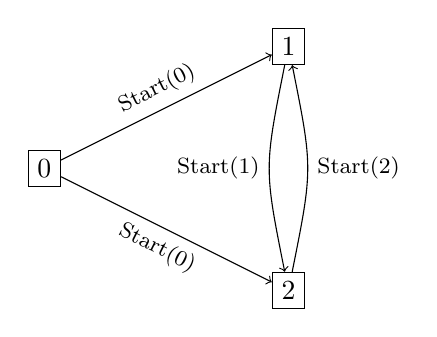
\begin{tikzpicture}[scale = 3.1]
\draw(0,0) node[draw](0) {\scalashape 0};
\draw(1.0, 0.5) node[draw](1) {\scalashape 1};
\draw(1.0, -0.5) node[draw] (2) {\scalashape 2};
\draw[->] (0) -- node[above,sloped]{\scalashape\labelSize Start(0)}  (1);
\draw[->] (0) -- node[below,sloped]{\scalashape\labelSize Start(0)}  (2);
\draw[->] (1) .. controls (0.9, 0) .. 
  node[left]{\scalashape\labelSize Start(1)} (2);
\draw[->] (2) .. controls (1.1, 0) .. 
  node[right]{\scalashape\labelSize Start(2)} (1);
\end{tikzpicture}%
\end{minipage}

\smallskip

More generally, each node ignores every |Start| message it receives other than
the first (but it won't expect a subsequent |Finished| message).  If node |n1|
receives a message |Start(n2)| from |n2|, then previously it sent a message
|Start(n1)| to~|n2|, which |n2| will also ignore.  The edge between |n1|
and~|n2| will not be included in the spanning tree, since both nodes will be
connected to the initiator~|0| by other edges, so that edge would erroneously
create a cycle.

The above example also illustrated that the system needs to use buffered
channels.  If we used synchronous channels in the above scenario, then when
nodes~|1| and~|2| try to send a message to each other, the system would
deadlock.  It is enough to use one-place buffered channels, since at most a
single message is sent on each channel.  It is tempting to try to avoid this
problem using an alternation, with each node willing to either send to
another, or receive from other nodes.  However, this violates the usage rule
for alternations that both ports of a channel may not be simultaneously
feasible in alternations.

Figure~\ref{fig:spanning-tree-node} defines a node with identity~|me|.  The
node has an array~|ins| of in-ports, and an array~|outs| of out-ports: these
should be indexed consistently, so |ins|$(i)$ and |outs|($i$) connect to the
same node.

%%%%%%%%%%

\begin{figure}
\begin{scala}[numbers=left]
  private def node(me: Int, ins: Array[??[Msg]], outs: Array[!![Msg]]) 
  = thread(s"node($me)"){
    val size = ins.length; require(outs.length == size); var edges = List[Edge]()
    if(size != 0){
      // Identity of this node's predecessor, and its index in the arrays.
      var pred = -1; var pIx = -1; var terminated = false
      // Waiting phase.
      if(me != 0) attempt{
        alt( | (  £\label{line:waiting}£
          for(i <- 0 until size)
          yield ins(i) =?=> { case Start(p) => pred = p; pIx = i }
        ) )
      }{ terminated = true } // This node is not connected. 
      if(!terminated){
        // Sending phase. 
        for(i <- 0 until size; if i != pIx) outs(i)!Start(me)£\label{line:sending}£
        // Receiving phase.
        val pending = Array.fill(size)(true); if(pIx >= 0) pending(pIx) = false
        serve( | ( £\label{line:receiving}£
          for(i <- 0 until size)
          yield pending(i) && ins(i) =?=> { m =>
            m match{
              case Finished(es) => edges = es++edges
              case Start(_) => {} // Ignore this message.
            }
            pending(i) = false
          }
        ) ) // end of £serve£.
        // Finishing phase.
        if(pIx >= 0) outs(pIx)!Finished((pred,me)::edges) £\label{line:finished}£
      } // end of £if(!terminated)£.
    } // end of £if(size != 0)£.
    if(me == 0){
      result = edges
      for(i <- 0 until n; j <- 0 until n){ £\label{line:close}£
        val c = chans(i)(j); if(c != null) c.close()
      }
    } 
  }
\end{scala}
\caption{A node in the spanning tree example.}
\label{fig:spanning-tree-node}
\end{figure}

%%%%%%%%%%

A node other than node~|0| starts (from line~\ref{line:waiting}) by waiting to
receive a |Start| message, recording the identity and index of its
predecessor.  (We explain the use of the |attempt| construct below.)

The node then sends a |Start| message to each of its neighbours in the graph
other than its predecessor (line~\ref{line:sending}).  

Next, the node waits (from line~\ref{line:receiving}) to receive |Finished|
messages from those nodes.  It accumulates the edges of the subtree in the
list~|edges| (see Scala box~\ref{sb:lists}).  As discussed above, if it
receives a |Start| message during this phase, it ignores it.  It uses a bitmap
|pending| to record the indices of neighbours from which |Finished| (or
|Start|) messages are pending.  The |serve| loop terminates when all entries
in |pending| are false.

Finally (line~\ref{line:finished}) it sends the accumulated subtree to its
predecessor (other than for the initiator).  The initiator,  node~|0|, stores
the resulting subtree in the object variable~|result|, which will allow it to
be returned subsequently.

It is possible that the graph is not connected, in which case nodes that are
not reachable from node~|0| will still be waiting at line~\ref{line:waiting}
to receive a |Start| message.  Node~|0| closes all the channels
(line~\ref{line:close}) to allow the threads to terminate. 

As a small optimisation, any node that has no neighbours shortcuts most of the
code.

%%%%%%%%%%

\begin{figure}[hbtp]
\begin{scala}
  import scala.collection.mutable.ArrayBuffer

  def apply(): List[Edge] = {
    // Initialise channels: £chans(i)(j)£ is from £i£ to £j£.
    for(i <- 0 until n; j <- 0 until n; if adjacency(i)(j)){
      assert(i != j && adjacency(j)(i))
      chans(i)(j) = new OnePlaceBuffChan[Msg]
    }
    // In£-£ports for node £i£.
    def mkIns(i: NodeId): Array[??[Msg]] = {
      val ins1 = new ArrayBuffer[??[Msg]]
      for(j <- 0 until n; if adjacency(i)(j)) ins1 += chans(j)(i)
      ins1.toArray
    }
    // Out£-£ports for node £i£.
    def mkOuts(i: NodeId): Array[!![Msg]] = {
      val outs1 = new ArrayBuffer[!![Msg]]
      for(j <- 0 until n; if adjacency(i)(j)) outs1 += chans(i)(j)
      outs1.toArray
    }
    run(|| (for(i <- 0 until n) yield node(i, mkIns(i), mkOuts(i))))
    result
  }
\end{scala}
\caption{The main code for the spanning tree example.}
\label{fig:spanning-tree-apply}
\end{figure}

%%%%%

Figure~\ref{fig:spanning-tree-apply} constructs the system.  It starts by
creating channels corresponding to each edge.  The helper functions |mkIns(i)|
and |mkOuts(i)| accumulate the in-ports and out-ports for node~|i| (using an
|ArrayBuffer|: see the online API documentation).  Finally, it constructs the
nodes, runs them, and returns the result that node~|0| stored in the |result|
variable.

%%%%%%%%%%

\begin{figure}
\begin{scala}
  def doTest = {
    val n = 2+Random.nextInt(10); val adjacency = Array.ofDim[Boolean](n,n)
    for(i <- 0 until n; j <- 0 until i; if Random.nextDouble() <= 0.3){ 
      adjacency(i)(j) = true; adjacency(j)(i) = true 
    }
    val tree = new SpanningTree(n, adjacency)()

    def errMsg = adjacency.map(_.mkString(", ")).mkString("\n")+"\n"+tree
    // Check £adjacency£ and £result£ are compatible.
    // £reached£ records the nodes reached by the tree.
    val reached = new Array[Boolean](n); reached(0) = true
    for((a,b) <- tree){
      assert(reached(a), s"Unreached source of edge: ($a, $b)\n"+errMsg)
      assert(!reached(b), s"Node reached by two paths: $b\n"+errMsg)
      assert(adjacency(a)(b), s"Non-edge used: ($a, $b)\n"+errMsg) 
      reached(b) = true
    }
    // Check no other node should have been reached.
    for(i <- 0 until n; if !reached(i); j <- 0 until n)
      assert(!(reached(j) && adjacency(i)(j)), s"$i not reached:\n"+errMsg)
  }
\end{scala}
\caption{Testing the spanning code example.}
\label{fig:spanning-tree-test}
\end{figure}

    %% // Count number reached.
    %% var numReached = 0; for(i <- 0 until n; if reached(i)) numReached += 1
    %% // Does `tree` have the right length to be a tree?
    %% assert(numReached == tree.length + 1, s"Not a tree.\n"+errMsg)

Figure~\ref{fig:spanning-tree-test} performs a single test on the program;
this can be repeated many times.  It chooses the number~|n| of nodes randomly,
and then constructs a random graph where there is an edge between nodes~|i|
and |j| (for $\sm i \ne \sm j$) with probability $0.3$.  It then uses the
spanning tree program to construct a purported spanning tree.  It then checks
the correctness of the result.  It traverses the list of edges, calculating
(using bitmap |reached|) which nodes are reached by the tree, and checks that
each edge joins a node already seen to a node not previously seen, and that
each such edge is an edge in the original graph.  Finally, it checks
that no further nodes could have been reached.
